\subsection{Interfaccia}
\begin{frame}
  \frametitle{Interfaccia}
  
  \begin{figure}
   \centering
   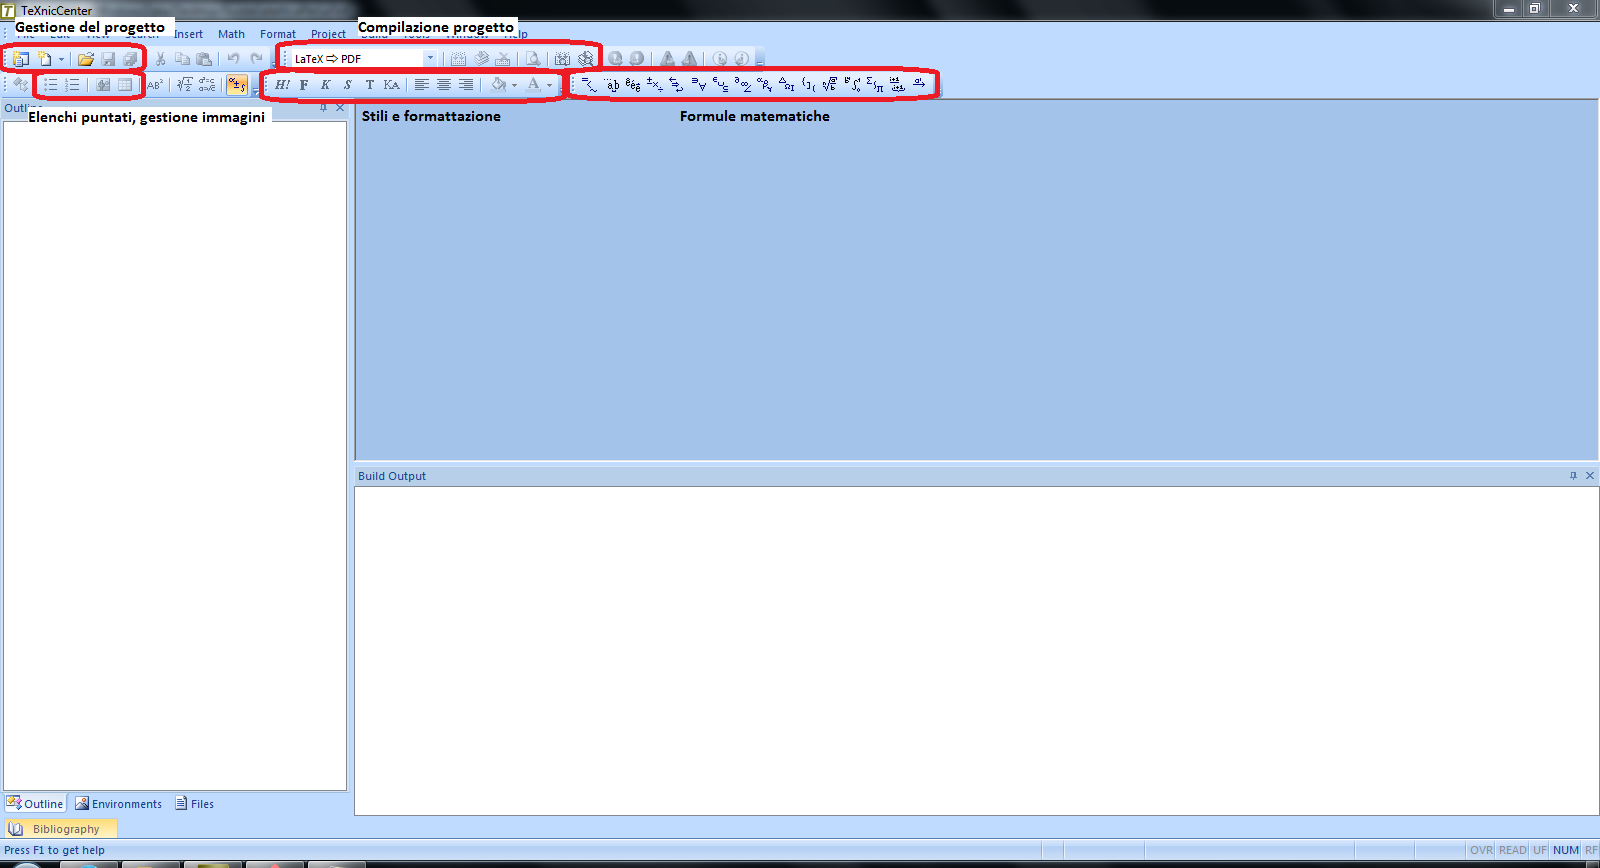
\includegraphics[scale=0.25]{texniccenterprincipale}
  \end{figure}
\end{frame}


\begin{frame}
  \frametitle{Interfaccia}
  
  \begin{figure}
   \centering
   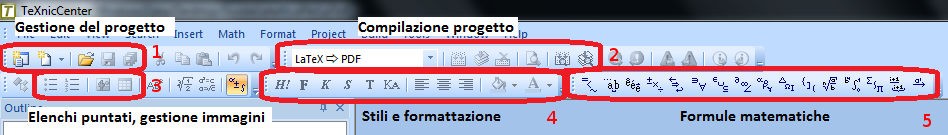
\includegraphics[scale=0.40]{texniccenterzoom}
  \end{figure}
  
  \begin{enumerate}
   \item Salvataggio, apertura documenti
   \item Compilazione del progetto, scelta dei formati di output
   \item Elenchi puntati, numerati, aggiunte immagini
   \item Stili e formattazione del testo
   \item Inserimento facilitato di formule matematiche
  \end{enumerate}

\end{frame}

\subsection{Creazione Progetto}
\begin{frame}
  \frametitle{Creazione Progetto}
  
    \begin{textblock*}{5cm}(9cm,3cm)
      
\includegraphics[scale=0.20]{AngryWalter}
    \end{textblock*}
    
    \huge Armiamoci di pazienza!
\end{frame}
